%!TEX root = ../template.tex
%%%%%%%%%%%%%%%%%%%%%%%%%%%%%%%%%%%%%%%%%%%%%%%%%%%%%%%%%%%%%%%%%%%
%% chapter1.tex
%% NOVA thesis document file
%%
%% Chapter with introduciton
%%%%%%%%%%%%%%%%%%%%%%%%%%%%%%%%%%%%%%%%%%%%%%%%%%%%%%%%%%%%%%%%%%%
\newcommand{\novathesis}{\emph{novathesis}}
\newcommand{\novathesisclass}{\texttt{novathesis.cls}}


\chapter{Introduction}
\label{cha:introduction}

\section{Motivation and context} %%%%%%%%%%%%%%%%%%%%%%%%%%%%%%%%
\label{sec:motivation_and_content}

Throughout the history of humanity, plant pests and diseases have been numerous times responsible for significant losses in society. Effects range from starvation, extinction of natural resources, negative impact on national/international resources or even deaths in a population.

Nowadays, pests and diseases do not present such threats but still constitute a relevant problem since they result in substantial losses to farmers by reducing the value of their products: yield loss, as studied in \cite{Kamilaris2017}\cite{Walker1983}. To minimize yield loss, there are two main approaches when handling plant pests and diseases: \emph{Prevention and Treatment}.

Prevention is based on prediction models, field records or general management tactics that are applied before the plants are actually infected \cite{StuartB.Hill}. Treatment, on the other hand, is all about deploying active substances to fight the already present disease. Prevention is obviously the preferable option when handling pest control since it represents no yield loss and no chemicals are used.

This dissertation, while focusing on prevention, proposes a framework/methodology for data collection and visualization of outdoor farming fields. This means tracking the growth of the plants, the location and intensity of the pest, soil information and climatic conditions. Several pests will be studied, but more than a system to fight specific pests (or pests in specific cultures), a framework that may be used to study the connections between Botany (the cultivated plant species), Entomology (parasite species), soil and climatic conditions will be created. 

During the development of this dissertation, the \emph{Fitoagro} project will be used as a case study of the methodology. \emph{Fitoagro}, as an Operational Group, consists of several partners with a common interest in a specific, practical innovation project: Pest Monitoring for the Apple and Pear Cultures in West Portugal. The people involved in the Operational Group come from a diverse combination of practical and scientific backgrounds (farmers, scientists, agri-business and others). Below are listed the main partners of the Fitoagro project.

\begin{description}
	\item [COTHN] Centro Operativo e Tecnológico Hortofrutícola Nacional
	\item [FCT/UNL] Faculdade de Ciências e Tecnologia da Universidade Nova de Lisboa
	\item [ISA] Instituto Superior de Agronomia
	\item [ESAS] Escola Superior Agrária de Santarém
	\item [ESACB] Escola Superior Agrária de Castelo Branco
\end{description}

Other entities such as agricultural cooperatives will also directly contribute as associates of the COTHN national entity, mainly in the data-collection process and the study of the biological species present in their very own farming fields. These above-listed organisations work together on specific and practical solutions to the following emerging pests (harmful ectoparasites):

\begin{enumerate}
	\item \textit{Dasineura pyri (Bouché)}
	\item \textit{Aphanostigma pyri}
	\item \textit{Stemphylium vesicarium}
	\item \textit{Pseudococcus viburni / Planococcus ficus}
\end{enumerate}

To successfully study a species, a significant amount of data is needed. That being said, if the current farming season brings new pest species with a decent number of samples, they will be considered to the study.

With features ranging from data collection to a visual monitoring system, the FitoAgro system will be able to visually empower producers and farmers to make better decisions when protecting their assets from pests and diseases. A couple of research questions waiting to be answered are "Can we detect a geographic pattern in a pest's behaviour?" or "Can the data collection process of pest occurrences be automated?". 

% section motivation_and_content (end) %%%%%%%%%%%%%%%%%%%%%%%%%%%%%%%%


\section{Problem} % (fold) %%%%%%%%%%%%%%%%%%%%%%%%%%%%%%%%
\label{sec:problem}

\subsection{Historical background and World Population Growth} % (fold)
\label{subsec:historical_background}

The first agricultural revolution came along during the advent of increased mechanization, from 1900 to 1930. Each farmer produced enough food to feed about 26 people during this time \cite{DongoskiRob}.
%
The 1990s prompted the Green Revolution with new methods of genetic modification, which led to each farmer feeding about 155 people.
%
It is expected that by 2050, the global population will reach about 9.6 billion \cite{DESA2015}, and food production must effectively double from current levels in order to feed every mouth. With new technological advancements in the agricultural revolution of precision farming, each farmer is expected be able to feed 265 people on the same acreage \cite{DongoskiRob}.

Digital agriculture is widely recognized as the third great revolution of modern agriculture. The introduction and implementation of mechanization (1900 to 1930) and genetic modification (1990 to 2005) are referred to as Ag 1.0 and Ag 2.0 respectively. Both revolutions drove efficiency, yield and profitability to levels previously unattainable, and are now conventional in developed countries across the world.

While Ag 1.0 and Ag 2.0 definitely drove significant changes in agriculture, Ag 3.0 will be the most transformative and disruptive, not only on the farm, but across the entire agriculture and food value chain \cite{Lewis&ClarkVentures}.

\subsection{The ever going study of Pest}
\label{subsec:evergoing_study_pest}

A Pest is any plant or animal detrimental to humans or human concerns including crops, livestock, and forestry. In its broadest sense, a pest is a competitor of humanity. Pests are usually categorized by taxon. Different taxonomies are usually studied by different branches of Biology. 

The term "plant pest" has a specific definition in terms of the \textit{International Plant Protection Convention} and phytosanitary measures worldwide. A pest is any species, strain or biotype of plant, animal, or pathogenic agent injurious to plants or plant products. 

Pest and disease study is, obviously, a continuous field of study since human interaction keeps disturbing nature's balance, which eventually leads to mutations, migrations, species. Plant pests keep developing resistances against active substances used in the fields (pesticides). Pest species evolve pesticide resistance via natural selection: the most resistant specimens survive and pass their genetic traits to their offspring. Although the evolution of pesticide resistance is usually discussed as a result of pesticide use, it is important to keep in mind that pest populations can also adapt to non-chemical methods of control.

Speciation (repeated formation of new species) leads to a hierarchical structure of the same species that developed specific traits for each culture it threatens. According to \cite{Sharma2014} pest life cycles are also changing so their first seasonal appearance is gradually evolving over time. All the above-mentioned factors contribute to the idea that pest control is still a problem, and Nature makes sure of that. Proper models have to constantly be built for new species, new traits, different conditions etc. 


\subsection{Spreadsheets}

Even though the problems mentioned in \ref{subsec:historical_background} and \ref{subsec:evergoing_study_pest} stand as important, there is a more practical and urgent problem.

Technological advances offer tools to farming management tools, mostly by providing a data collection system: weather and Soil stations display their readings on proprietary web interfaces. Biological Measurements however are tracked using paper spreadsheets which are afterwards uploaded to a document-sharing service like \textit{Google Drive}. While acceptable for small farms and direct measurement analysis ("Is the temperature above 40ºC in the field?"), it is hard to build logic that combines weather, soil and enemy-tracking data that can sucessfully draw conclusions.

These paper spreadsheets are used \emph{in-situ} and track phenological stages of the crop, enemy observations, dates of phytopharmaceutical product applications and production system data. An enemy observation spreadsheet for a single farming field is available in \ref{fig:spreadsheet}. On the spreadsheet, the \textit{Barrocalvo} farming field is sampled 4 times (dates on the table header) on different phenological stages for a specific enemy: Aphanostigma pyri. A1-A10 are the ten randomly selected trees being monitored. For each tree, 3 adhesive tapes are placed on the trunk(T) and 2 branches(P1 and P2). On the date column, zeros and ones are the counts for the enemy(insects) on the traps (adhesive tapes). 

Figure \ref{fig:spreadsheet} also shows a perfect example of how irregular the registering method is: on the 11th of April, in the trunk of the tree number seven, it is not clear how many enemies were tracked.

\begin{figure}[htbp]
  \centering
  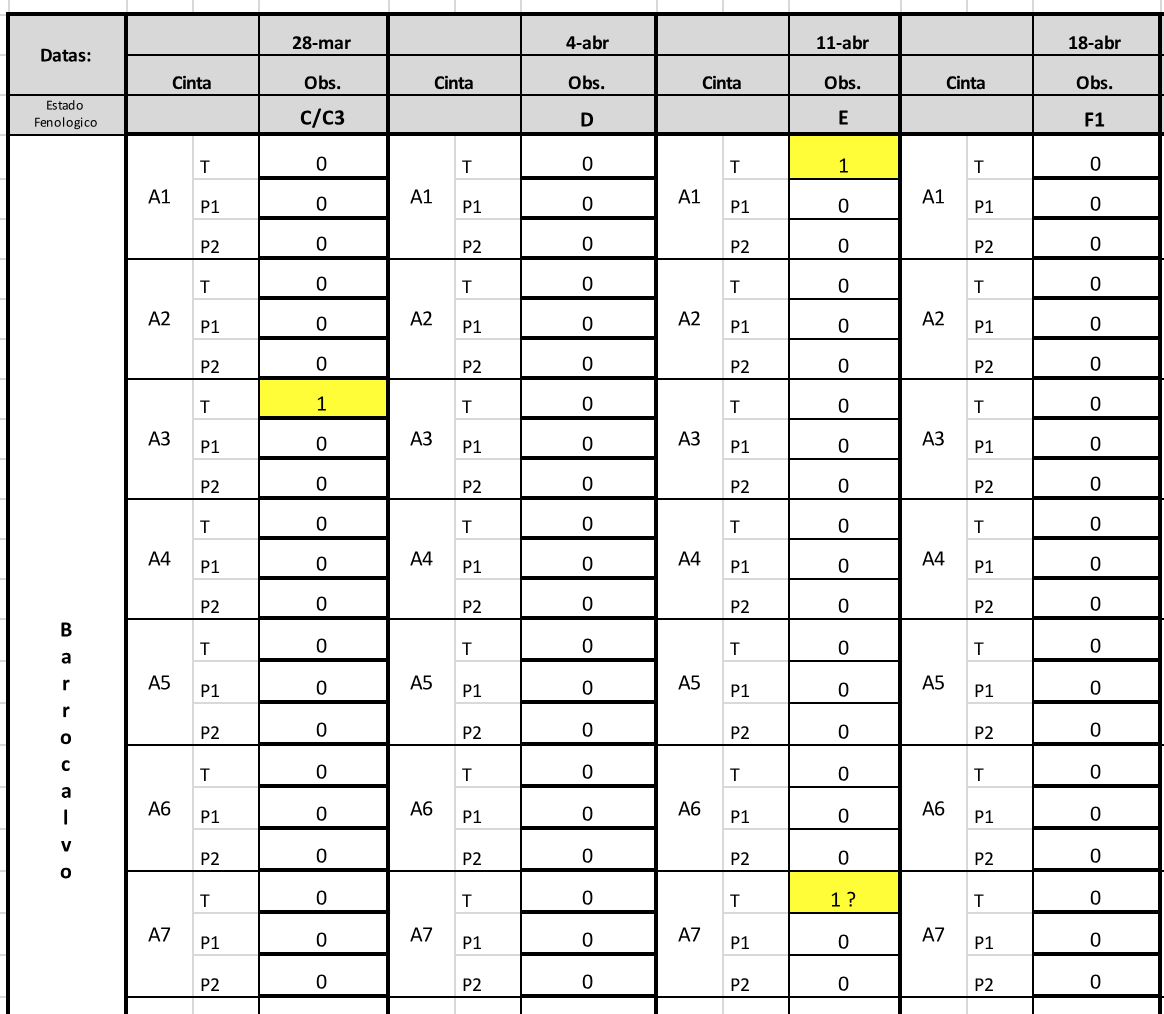
\includegraphics[width=0.85\linewidth]{spreadsheet}
  \caption{A sample from the collaborative spreadsheet for the \textit{Barrocalvo} farming field (FitoAgro project)}
  \label{fig:spreadsheet}
\end{figure}

More details on the use of these field-notebooks is available in chapter \ref{cha:problem}.

\section{Objectives} % (fold) %%%%%%%%%%%%%%%%%%%%%%%%%%%%%%%%
\label{sec:objective}

\subsection{Precision Agriculture}
\label{sec:precision_agriculture}

Precision Agriculture(PA) , Satellite Farming or Site-specific crop management (SSCM) is a key-component  of the third wave of modern agricultural revolutions (Ag 3.0). In it's essence, it is a farming management concept based on observing, measuring and responding to inter and intra-field variability in crops. Its main goal is to provide a decision support system for a whole farm management in order to optimize returns on inputs and, most importantly, preserving resources.

The basic principle of precision farming is an exact positional controlling of fertilisation, growth levels, pest presence, risk estimate or any other relevant key-performance indicator with the accuracy of a few meters. The whole process requires a big amount of data to be collected which enables the control of the management process. The better the data collection method, the more resolution data will have, which allows for better conclusions to be taken. Studies conducted on Precision Agriculture as \cite{Khanal2017} \cite{Talavera2017} \cite{Kruize2016} \cite{Culibrina2015} \cite{Jawad2017} \cite{Resu2015} \cite{Alam2014} \cite{JointResearchCentreJRCoftheEuropeanCommission2014} \cite{Mohanraj2016} \cite{Sankaran2010} \cite{Nip2003} show different approaches in data collection with different resolutions. Most of the recent efforts are incorporating \emph{IOT} (Internet of Things) in the agricultural domain leading to a plant-level analysis of the field. Most of the described sensor meshes, ul have high costs and therefore are not analised in chapter \ref{cha:state_of_the_art} since they do not present a reasonable choice for medium-scale independent producers such as the cooperatives from the FitoAgro project mentioned in \ref{sec:motivation_and_content}.

From the works listed above, Precision Farming is usually divided into the following steps:

\begin{description}
\item [Data Collection] Inter field systems collect data with a field-level of resolution. Increasing the number of sources provides a smaller scale analysis. Geolocating data sources enables the farmer to read a map of his property (henceforth called soil map) with the most important crop variables.
\item [Variables] The data collected can measure different things. Usually, climatic conditions (hail, drought, rain, etc.), soils (texture, depth, nitrogen levels), cropping practices (no-till farming), weeds and disease. Permanent indicators as weather stations, provide information about the main environmental constants. Point indicators allow them to track a crop’s status, i.e., to see whether diseases are developing, if the crop is suffering from water stress, nitrogen stress, or lodging, whether it has been damaged by ice and so on. This information may come from weather stations and other sensors (soil electrical resistivity, detection with the naked eye, satellite imagery, etc.). Soil resistivity measurements combined with soil analysis make it possible to measure moisture content. Soil resistivity is also a relatively simple and cheap measurement.
\item [Strategies] Once with soil maps, Strategies can be either predictive (Predictive Approach), where   based on history and static features of the field, the farmer takes decisions. The Control Approach, on the other hand, collects data regularly during the crop cycle to provide a better temporal resolution. Decisions may be based on decision-support models and/or the farmer.
\item [Implementing practices] If some decisions are to be trusted to an algorithm, Variable Rate Technology can help to administer variable rates of pesticides(biological or chemical), nutrients, water, etc. through Variable Rate Application (VRA). Map Based and Sensor Based VRA present two very different paths.
\end{description}	

These simple four steps present a methodology for the continuous management of the farming field.

The main objective of this dissertation is to combine the methodology from Precision Agriculture with Pest Control strategies and build a framework that geographically maps important variables of a farming field.

Available options for Data Collection are studied in detail in chapter \ref{sec:state_of_the_art_data}. They include data sources such as as soil, weather and biological readings from different sources regarding: cost, efficiency, resolution, limitations while focusing on the needs of the Pest study. This framework will enable the building of regional risk maps (geographic likelihood of yield loss) for any outdoor farming field. For the end-user of the framework, farmers, some visualization techniques will be applied to ease-out farm management tasks.

The resulting framework will be available through a mobile interface and should empower farmers to make better decisions while managing their property by displaying sensor data in a map visualization adjusted to the agricultural domain. 

% section problem_and_objective (end)

\section{Major Contributions} % (fold) %%%%%%%%%%%%%%%%%%%%%%%%%%%%%%%%
\label{sec:contributions}

\subsection{State of the Art as a Review of Recent Efforts}
\label{sec:review_recent_efforts}

The State of the Art presents a good contribution itself. By organising and cathegorising different techniques by data source it is expected to achieve a detailed analysis of the recent trends in outdoor data collection as well as pest control methodologies.

\subsection{A framework for data collection and visualization of a farming field}
\label{sec:digital_mapping_framework}

Farming fields have, by default, ideal conditions for the development of life. That's why they are farming fields. Plants, as the farmer's objective, greatly benefit from this. The problem is that parasite species may also be present, parasitizing whatever plant species is being cultivated in the field.

This creates both a difficult problem for the farmer but also an interesting problem for the study of specific species.

By capturing as many field variables as possible, a geographic model of the farming field can be built. Sensoring organic growth levels for both (plant and pest) species as well as climatic variables may empower farmers to make better decisions on their farming fields. If enough data is supplied, a broader geographic mapping of certain pests and plants could be achieved in a collaborative sense. This represents palpable knowledge and information: "Where are the best zones to plant X crop?" is just an example of a wide range of questions that could be answered with this much geo-referenced data.

The Fitoagro project will be used as a case-study of the developed framework. Solutions for proper tracking the species mentioned on \ref{sec:motivation_and_content} will be developed. This means that the framework will be used directly by 5000 farmers spread across 30 agricultural organizations (COTHN associates). The case study will be on specific cultures and locations but the framework should be ready to scale out with more species (plants and pests) and locations.

This type of farming field monitoring is not available to all farmers due to the cost of implementation. Since some pest species require specific equipment to be read/analyzed, some design thinking techniques will be used to ease out the data collection process into, hopefully, an effortless process for the farmer. 

\subsection{Field visualization}
\label{sec:field_visualization}

A big component of the framework described above is the end-user analysis of the data being processed by the system. Visualization is of the utmost importance when analysing the data, so, in order to communicate the geolocated data that is to be collected, a specific soil map visualization that tackles all the necessities of the Pest Control domain will be developed. The focus will be on minimizing the complexity of the interface so that, the farmer intuitively understands his farm at a glance. In a broad sense, Design and Usability meet big data. Examples of the visualization under development are acessible on chapter \ref{cha:approach_and_planning}.

\section{Document Structure} % (fold) %%%%%%%%%%%%%%%%%%%%%%%%%%%%%%%%
\label{sec:document_structure}

\begin{enumerate}
	\item Introduction - Motivation and context, a brief introduction to the problem, objectives and major contributions.
	\item Detailed Problem - Details of the problem briefly described in the Introduction.
	\item State of the Art - Previous works in this domain and their solutions. Organize by sections, keywords, results and exclusion criteria.
	\item Approach - What is going to be implemented, why and how.
	\item The framework - Explaining the methodology, beneficts and limitations.
	\item Development Planning - General planning of the development of the FitoAgro solution according to the framework developed.
	\item Design and Implementation - Specific design choices and implementation details.
	\item Testing and fixes - A/B Testing process description of the proposed framework \textit{in situ}.
	\item Conclusions - General conclusions, final remarks and future work.
\end{enumerate}

